
\begin{figure}[htbp]
     \centering
     		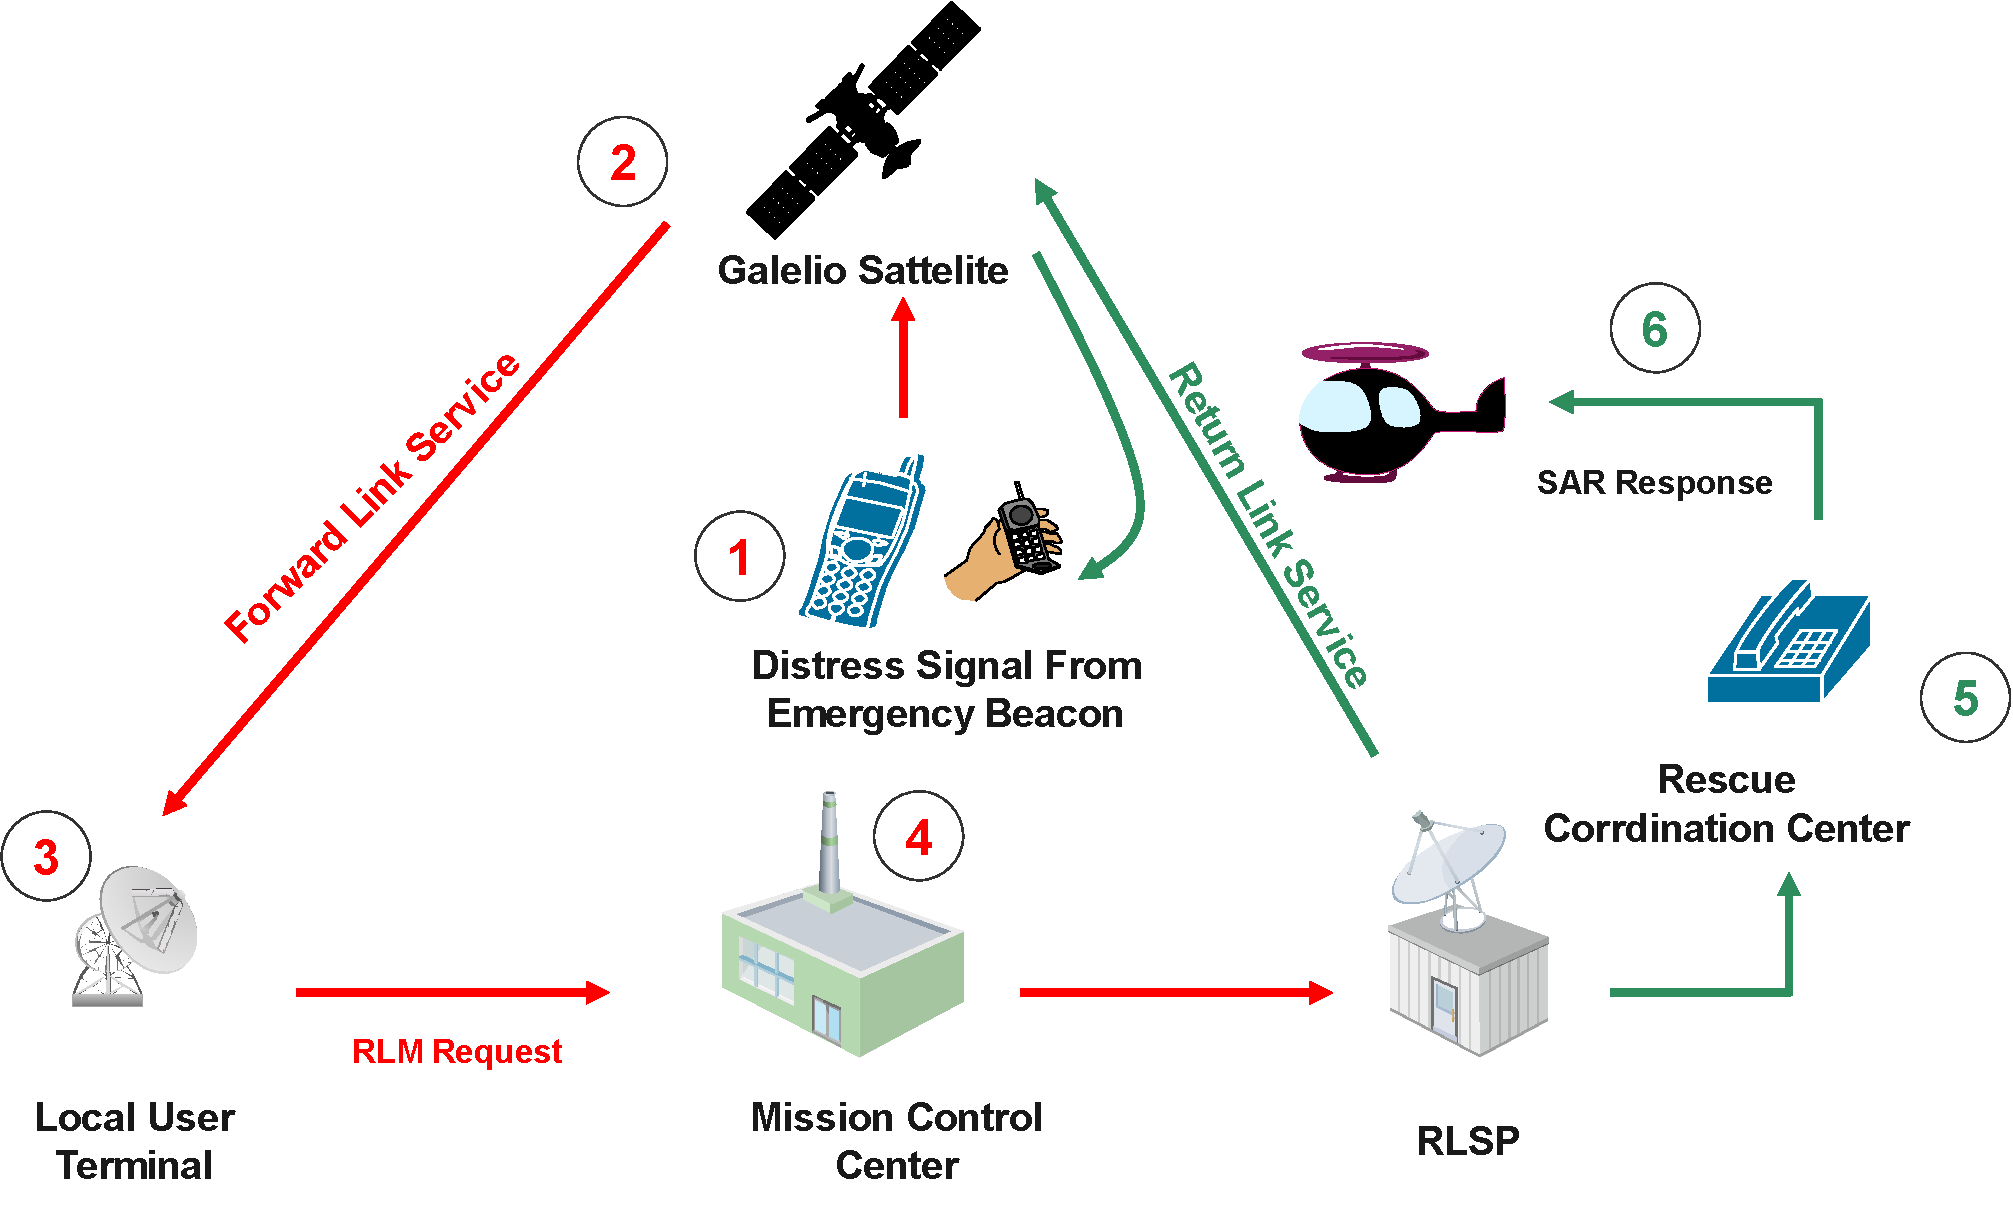
\includegraphics[width=320pt, height =200pt]{cs.pdf}
     \caption{SAR/Galileo Services \cite{galileoperformances,galileoossdd}.}
     \label{fig:usecase}
 \end{figure} 

\fig{fig:usecase} depicts the SAR/Galileo Services, illustrating the organizational structure of rescue services. The system encompasses multiple components that relay beacon signals from distressed users to rescue authorities. This section presents the system parameters and the formal response mode model.

\subsection{The system model}


COSPAS-SARSAT (C/S) is an international satellite-based Search and Rescue (SAR) distress alerting system established in 1979 by the USA, Canada, France, and the former USSR \cite{galileosarservice}.(See \fig{fig:usecase}). The full documentation is available in \cite{galileosarsdd}. The C/S system comprises:

\begin{enumerate}
    \item Beacons are 406 MHz radio transmitting devices employed in various applications. These include Emergency Position Indicating Radio Beacons (EPIRBs) and Ship Security Alert Systems (SSAS) for maritime use, Emergency Locator Transmitters (ELTs) and ELT Distress Tracking for aviation, and Personal Locator Beacons (PLBs) for individual use.

    \item The space segment \cmt{includes} satellites operating in low Earth orbit, geostationary orbit, and medium Earth orbit, responsible for processing signals transmitted by beacons.

    \item A Service Ground Segment (SGS) \cmt{consists of} a geographically distributed set of receiving ground stations known as Local User Terminals (LUTs). This network provides ground segment coverage, \cmt{allowing} the tracking of satellites and the generation of independent location estimates for user beacons.

    \item Mission Control Centers (MCC) are crucial in distributing C/S distress alerts globally and configuring the alerts for optimal response.

    \item The Sar/Galileo Ground Segment \cmt{consists of} five Reference Beacons (REFBE). These reference beacons \cmt{distibuted across} the European coverage Area are used to monitor the performance of the SAR/Galileo Service.
\end{enumerate}

The Galileo Search and Rescue (SAR) Forward link service is capable of receiving signals emitted by C/S compatible 406 MHz distress beacons (Forward Link Alert Message, as FLAM)and relaying this information to a ground segment network, known as the Local User Terminal (LUT), which consists of geographically distributed facilities deployed worldwide. The Return Link Service (RLS) enables the relay of data (Return Link Messages, or RLMs) back to the originating beacon. A primary function of the RLS is to provide the end-user of a distress beacon with automatic acknowledgment, confirming the detection of the alert and the determination of their location by the Search and Rescue (C/S) system.

Upon estimating the beacon's location, the Mission Control Center (MCC) issues an RLM\_Request. This request, covering the beacon's confirmed position, is transmitted to a backup MCC (Spanish or French). Subsequently, the RLS generates an RLM Transmission Request (RLMR) based on the original FLAM. The Galileo Core infrastructure processes the RLMR and uplinks the RLM to \cmt{appriopriate} Galileo \cmt{satellites, wich then} is broadcast to the originating beacon.

\cmt{Once the beacon receives the RLM}, sets \cmt{a} receipt status flag within FLAM. This status flag is then transmitted to the RLSP via the C/S MCC. \cmt{After} the RLSP acknowledges the receipt of the RLM, the Galileo system \cmt{stops sending} further \cmt{RLMs} to the beacon. However, if no acknowledgment of RLM reception is received within 24 hours of the initial RLM request, the Galileo system \cmt{will continue} to transmit RLMs to the beacon.

\subsection{Operational capabilities characteristics}



According to \cite{galileoperformances} and \cite{galileoossdd}, Galileo satellites \cmt{demonstrate} a reliability exceeding 88\% over a 12-year lifespan \cmt{, with} an availability of 99.5\%. \cmt{The work in} \cite{galileoosperformancereport} \cmt{reports that the availability of healthy signals from Galileo is 99.22}\%, with a recovery time of less than 15 hours. \cmt{This emphasizes the importance of ensuring timely service recovery}. Detection performance, a \cmt{crucial} aspect of the system, \cmt{refers to} the probability of successfully detecting 406 MHz beacon transmissions within the SAR/Galileo coverage area and receiving a valid beacon message at the SAR/Galileo LUT Facilities.

Three service states are defined for the SAR Forward link service in the ECA (European Coverage Area): Nominal, Degraded, and Severely Degraded. Nominal indicates normal operation. Degraded is characterized by either non-operational status for less than 24 hours continuously or less than 48 hours cumulatively over a calendar month or by losing communication with one or two ground segments (LUTs) for more than one day, or only 1 REFBE is in nominal status, or no REFBE is operational for less than 5 continuous days. Severely Degraded occurs when the SGS is non-operational for more than 24 hours continuously or more than 48 hours cumulatively over a calendar month or when communication is lost with all three LUTs and MCCs for more than four hours.

Similarly, the RLS has three service states: Nominal, Degraded, and Severely Degraded. The system is considered \quot{Degraded} if the RLSP is in degraded status or not operational for up to 7 cumulative hours within a calendar month or if RLM messages are delivered but not compliant with the latency MPL: The RLM Delivery Latency within 15 min was above or equal to 99.95\% \cite{galileoperformances}) which means that the Failure Rate is 0.05\%, and thus MTTF  is 2000 hours. \quot{Severely Degraded} status applies when the RLSP is not operational for more than 7 cumulative hours within a calendar month or if RLM messages are not delivered for more than 7 hours. In addition, based on the given availability of 99.8\% and the assumption of a very high MTBF, the estimated MTTR for the RLS would be approximately 500 hours.

\subsection{Formal modeling}

\begin{figure}[htbp]
     \centering
     		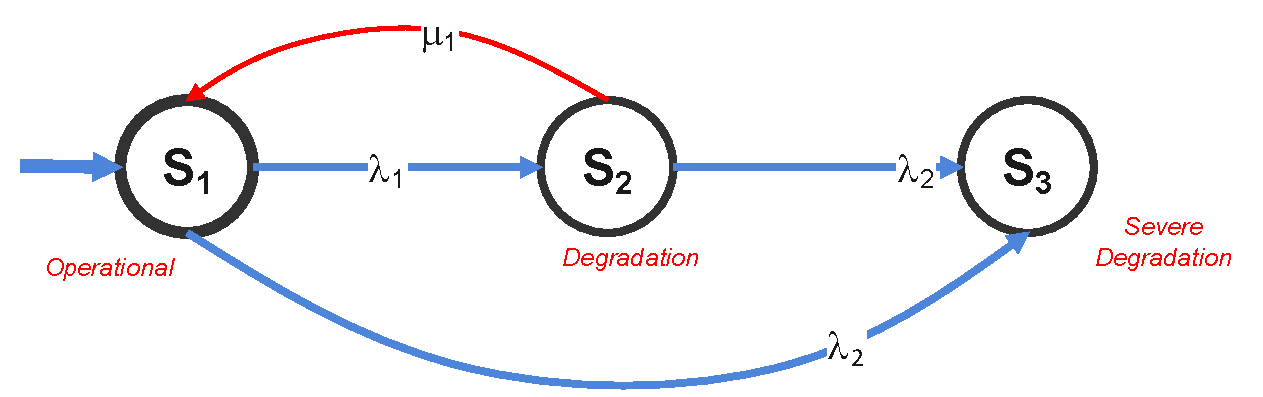
\includegraphics[width=250pt, height =80pt]{automat.pdf}
     \caption{Markov Model Pattern for SAR/Galileo Services.}
     \label{fig:model}
 \end{figure} 
 
The SAR/Galileo system can be modeled as a three-state Markov chain, illustrated in \fig{fig:model} and portrayed in the PRISM textual representation in \lst{exampleinprismtest}. State  \emath{S_{1}} represents the fully operational system, \cmt{while state} \emath{S_{2}} \cmt{indicates} a faulty state requiring recovery. State \emath{S_{3}} \cmt{signifies} a severe degradation state where maintenance is required. In the PRISM model, the system states are represented by an integer variable \emath{S}, which can take values from 0 to 3 (line 13). The assignment of degradation status relies on the constant values defined in lines 2-5. In this model, \emath{\lambda} represents the failure rate of system components, and \emath{\mu_{1}} \cmt{indicates} the recovery with repair rate. We \cmt{assume that the rates of} constant degradation and severe degradation rates (failure) follow a Poisson process. In \lst{exampleinprismtest}, the parameters are parametrizable as defined in lines 8-10. The reference documentation includes \cmt{various} sources of failure; \cmt{allowing the} model to be parametrized \cmt{so that users can} select which failures \cmt{impact} the communication system. \cmt{Additionally, this paper discusses how human reliability in sending rescue signals is} influenced by their psychological status, which we also model using a Poisson distribution. 



\lstdefinestyle{framed}
{
	frame=lrb,
	mathescape,
	numbers=left,
	belowcaptionskip=-1pt,
	xleftmargin=3.11em,
	xrightmargin=0.03cm,
	framexleftmargin=3em,
	framexrightmargin=0pt,
	framextopmargin=5pt,
	framexbottommargin=5pt,
	framesep=0pt,
	rulesep=0pt,
	numbers=left,
}

\lstset{
    breaklines=true,
    style=framed,
    escapeinside={<@}{@>},
    morekeywords={void, int, public, private, class, protected, submodules, network, connections, const, init, int, bool, double, module, rewards, endrewards, endmodule,label,ctmc},
    basicstyle=\small\ttfamily,
    keywordstyle=\bfseries\color{blue},
    morecomment=[f][\color{green!70!black}][0]{/*},
    morecomment=[l][\color{green!30!black}]{//},
    label=queueemodel
}

\begin{figure}[!htb]
\begin{minipage}{12.3cm}
\begin{lstlisting}[style=framed,
	caption=The System Status Over Execution Time,
 	label=exampleinprismtest]
ctmc    
//System states
const int Operational = 2;
const int Degraded = 1;
const int Severely_Degraded = 0;

//System performance rates
const double $\lambda_{1}$;
const double $\lambda_{2}$;
const double $\mu_{1}$;
//PRISM module
module Degradation
 S : [0..3] init Operational;
 [degradation]       S>0       $\rightarrow \lambda_{1}$:(S'=Degraded); 
 [sever_degradation] S>0       $\rightarrow \lambda_{2}$:(S'=Severely_Degraded); 
 [reset]             S=Degraded$  \rightarrow \mu_{1}$:(S'=Operational); 
endmodule

\end{lstlisting}
\end{minipage}
\end{figure}
